\chapter[Trigger Scintillator Counters]{Trigger Scintillator Counters
  \footnote{
    $CVS~revision~ $Id: scin.tex,v 1.9 2003/12/13 06:23:38 gen Exp $ $
  }
  \footnote{Authors: Robert~Feuerbach~\email{feuerbac@jlab.org},
    Bogdan~Wojtsekhowski~\email{bogdanw@jlab.org}}
}
\section{Overview}

\newcommand{\unit}[1]{\,\mbox{\ensuremath{\mathrm{#1}}}}

In the standard detector configuration each HRS has two trigger
scintillator planes, S1 and S2. The paddles in each plane are arranged to
provide segmentation along the detector-x direction. An additional
un-segmented scintillator plane, S0, can optionally be inserted into the
detector stack for experiments that require a high hadron trigger
efficiency. Fast signals from
these planes are used to form the trigger, as well as providing timing
information useful for particle identification.  Typically a coincidence between
two-or-more scintillator planes is used to form the trigger, and
through different combinations the triggering effiency of each plane can
be measured.

\infolevfour{
\begin{figure}[tbh]
  \begin{center}
    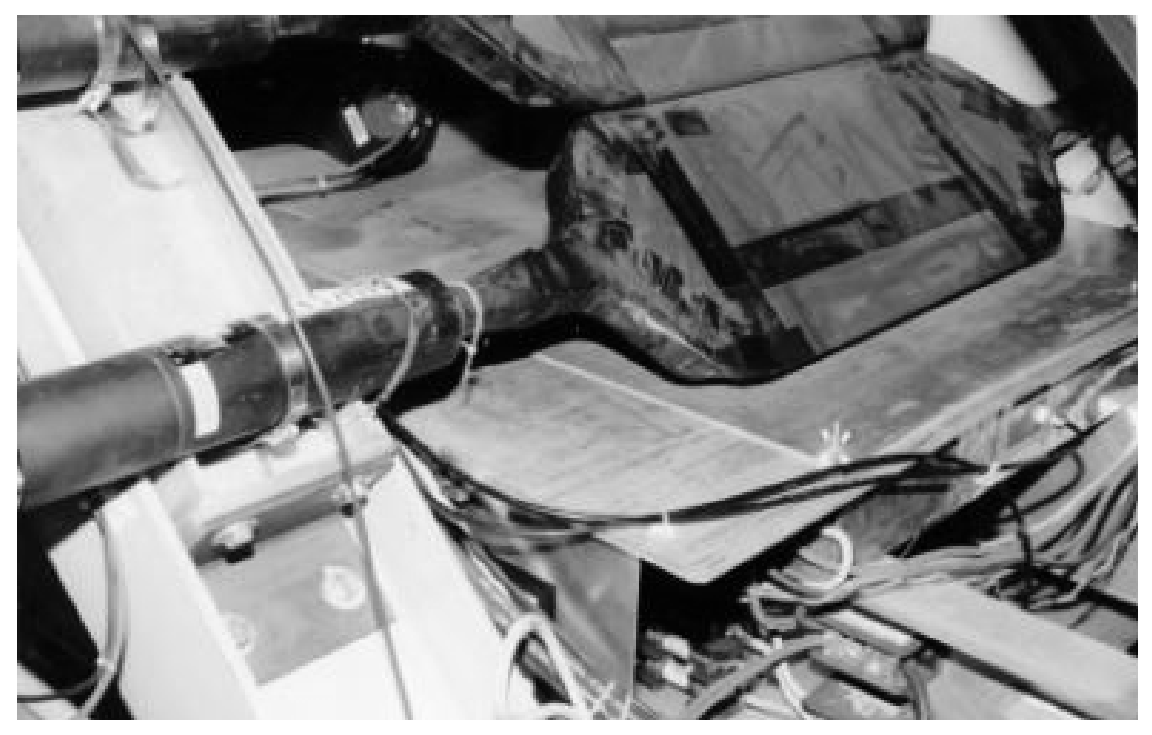
\includegraphics[width=.8\textwidth]{scint_fig5}
    \caption[Detectors: S1 Mounting]{S1 mounting}
    
    \label{fig:s1mount}
  \end{center}
\end{figure}
} % infolev
The S1 scintillator plane consists of six paddles, each with an active area
of 29.5~cm by 35.5~cm. The counters are made of 5~mm thick BICRON 408
plastic scintillator and use multi-strip adiabatic light guides which end
in a long cylindrical spool. There is an inlet for optical fiber mounted on
the side of the cylindrical light guide. Each paddle is viewed by a 2"
photo multiplier tube (Burle 8575) on each end.  The S1 paddles are
installed at a small angle to the S1-plane and overlap by 10 mm.  The
detectors are clamped to the detector frame through an additional A1
channel, and supported from the PMT housings. 
\infolevfour{Figure ~\ref{fig:s1mount} shows the mounting scheme for S1.
}%infolev
Signals from the PMTs are sent to Camac
modules on the second level of the shielding hut for processing.

\begin{figure}[tbh]
  \begin{center}
    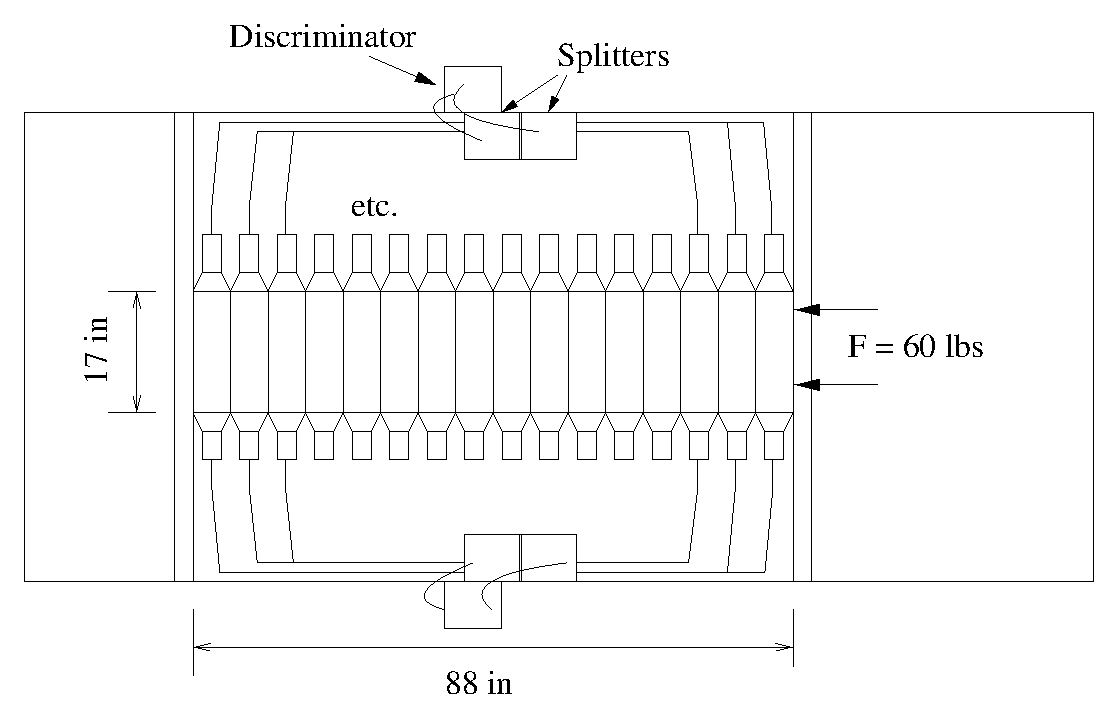
\includegraphics[angle=0,width=.8\textwidth]{scint2_layout}
    \caption[Detectors: S2 Layout]{The layout on the frame of the S2 paddles and
    electronics.}
    \label{fig:s2layout}
  \end{center}
\end{figure}

The S2 plane (also called S2m) consists of sixteen bars mounted on a steel
frame, as shown in Figure~\ref{fig:s2layout}. The bars are made a fast
plastic scintillator (EJ-230) with dimensions of 17\unit{in} by
5.5\unit{in} by 2\unit{in} thick. Since the S2 detector is located after
the tracking and PID detectors in the HRS, the extra material does not
compromise the particle detection while providing a greater photon yield
for an improved timing resolution as compared to S1. The bars are
individually wrapped with 25\unit{\mu m} of mylar and 50\unit{\mu m} of
black tedlar. The bars do not overlap, but are pressed together by a force
60~lbs to minimize the dead area between adjacent bars. Trapezoidal lucite
light guides on both ends couple the bar to 2" photo multiplier tubes
(Photonis XP2282B). S2 is assembled on a sub-frame mounted on rails in the
detector frame. The bars are supported by two thin aluminimum honeycomb
panels placed over the scintillators, leaving the PMTs and bases accessible
for servicing. On the frame are mounted analog splitters and threshold
discriminators for the initial signal processing.

The optional S0 plane is made of 10~mm thick BICRON 408 plastic
scintillator with an active area 170~cm long by 25~cm wide. This area is
covered by a single paddle, viewed from each end by 3" PMTs (XP4312B). The
signals from these PMTs are sent to Camac modules on the second level of
the shielding hut for processing.

\infolevone{
  \section{PMT regime and time resolution}
  
  High energy electrons passing perpendicular to the S1 detector plane yield
  about 400-500 photons at the photo cathode of each PMT. In a fresh
  PMT this leads to 80-100 photo electrons. On the HRS the discriminators
  have a threshold of 45 mV and a typical PMT has gain $~ 3*10^6$. The HV for
  a fresh PMT should be in the range -1800 to -2000 V. Based on PMT pulse rise
  time ( 2.8 ns ) and photo electron statistics the time resolution for the
  counter is about $\sigma_t \approx 0.2\unit{ns}$.
  The propagation time of the light inside the detector is about 10 ns, which
  needs to be corrected by using track position information.
  
  Due to its thicker cross-section, the initial photon yield in S2 is larger
  than in S1. With cosmic rays around 900 photo electrons per PMT were
  observed. To match the gains, the HV on the PMTs were adjusted, and
  set between -1700 and -2000 V.  The signals from each PMT are sent
  to a passive 90/10\% splitter, with the greater and lesser portions sent to
  the on-frame discriminator and Fastbus ADCs,respectively. The
  discriminator is a Phillips-Scientific model 706 with the threshold set
  at 10mV. Both NIM outputs are used on each channel, 
  with one line as input for the trigger-logic and the other going to a TDC
  after passing through a NIM-ECL converter and a delay of some 880ns. The
  average resulting timing resolution for a single PMT was measured to be
  better than $\sigma_{pmt} < 150\unit{ps}$.

  The geometry of S0 counter limits its timing resolution. In 1999
  the resolution was measured to be $\sigma_t \approx .2\unit{ns}$.
  
  LeCroy HV 1460 modules are used to supply HV power for the trigger
  counters. The HV can be controlled from a VT100 terminal connected through
  a terminal server or through the EPICS~\cite{EPICSwww} system based on the HAC computer.
  Current HV settings for the trigger counters should be found from a
  printout of the EPICS control in the last experimental logbook.
  
}

\infolevtwo{
  Figures ~\ref{fig:scinhv} and ~\ref{fig:s1scinhvc} give examples which are included
  for guidance only. The settings used in the plots may be not correct.
  
  \begin{figure}[p]
    \begin{center}
      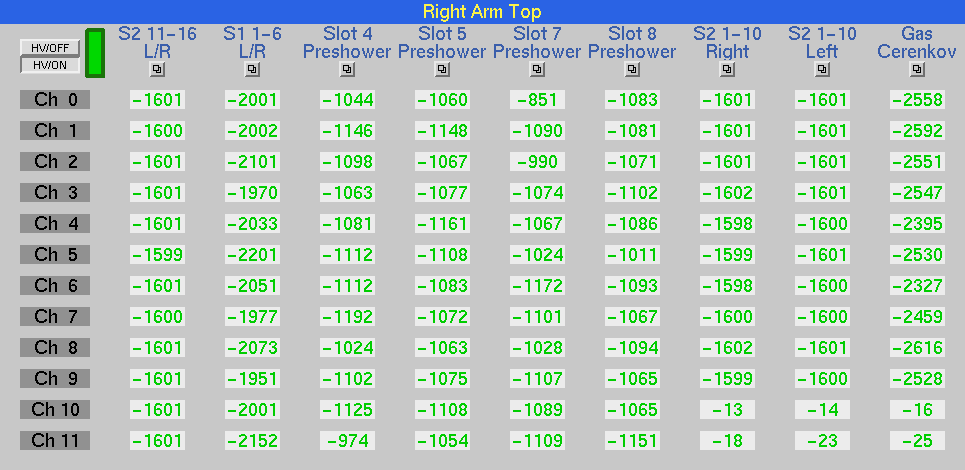
\includegraphics[width=.8\textwidth]{medm_halla_hv_rhrs3}
      \caption[Detectors: HV HRSR Summary Screen]{EPICS HV HRSR summary screen.}
      \label{fig:scinhv}
    \end{center}
  \end{figure}
  
  \begin{figure}[p]
    \begin{center}
      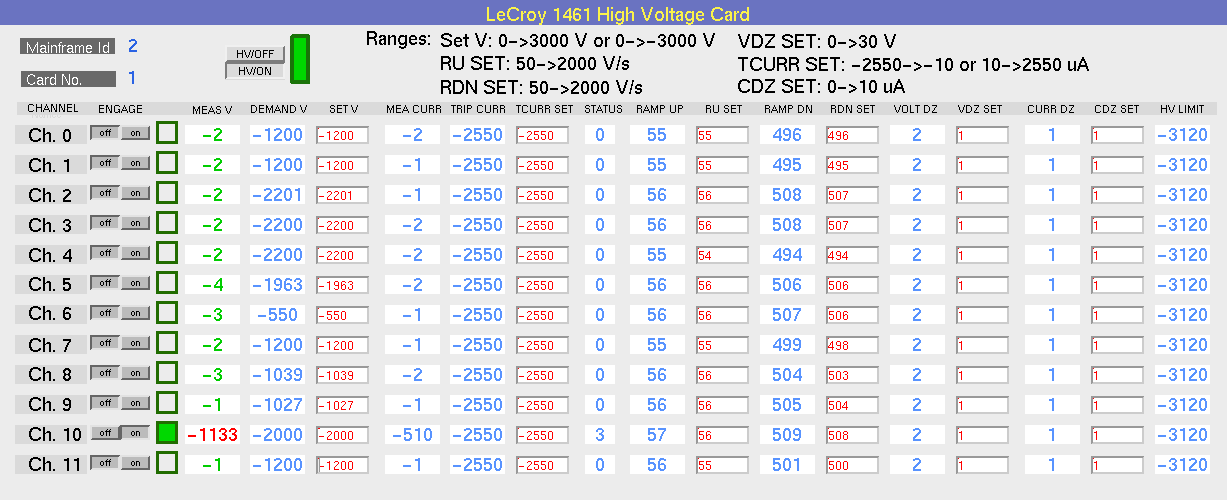
\includegraphics[width=.8\textwidth]{medm_halla_hv_card}
      \caption[Detectors: HV Screen for Single Card]{HV screen for a
	single card.}
      \label{fig:s1scinhvc}
    \end{center}
  \end{figure}
  
}

\infolevone{
  \section{PMT operation monitoring}
  
  There are two ways to monitor PMT/detector performance. The first is based
  on a scaler display program which provides information about PMT counting
  rates and coincidence counting rates.  A large variation of the rates
  between paddles is an indication of a possible problem. The second
  technique is to track the average amplitudes of each PMT for good track
  events after a complete event reconstruction.  For high efficiency of the
  trigger it is important to keep the average amplitude for the S1 PMTs above
  600 channels. Due to the passive splitting, the S2 amplitudes should be
  expected to be only about 50 channels above the pedestal.

%\clearpage
  
  \section{Measures to Protect the PMTs from Helium}
  
  \begin{figure}[tbh]
    \begin{center}
      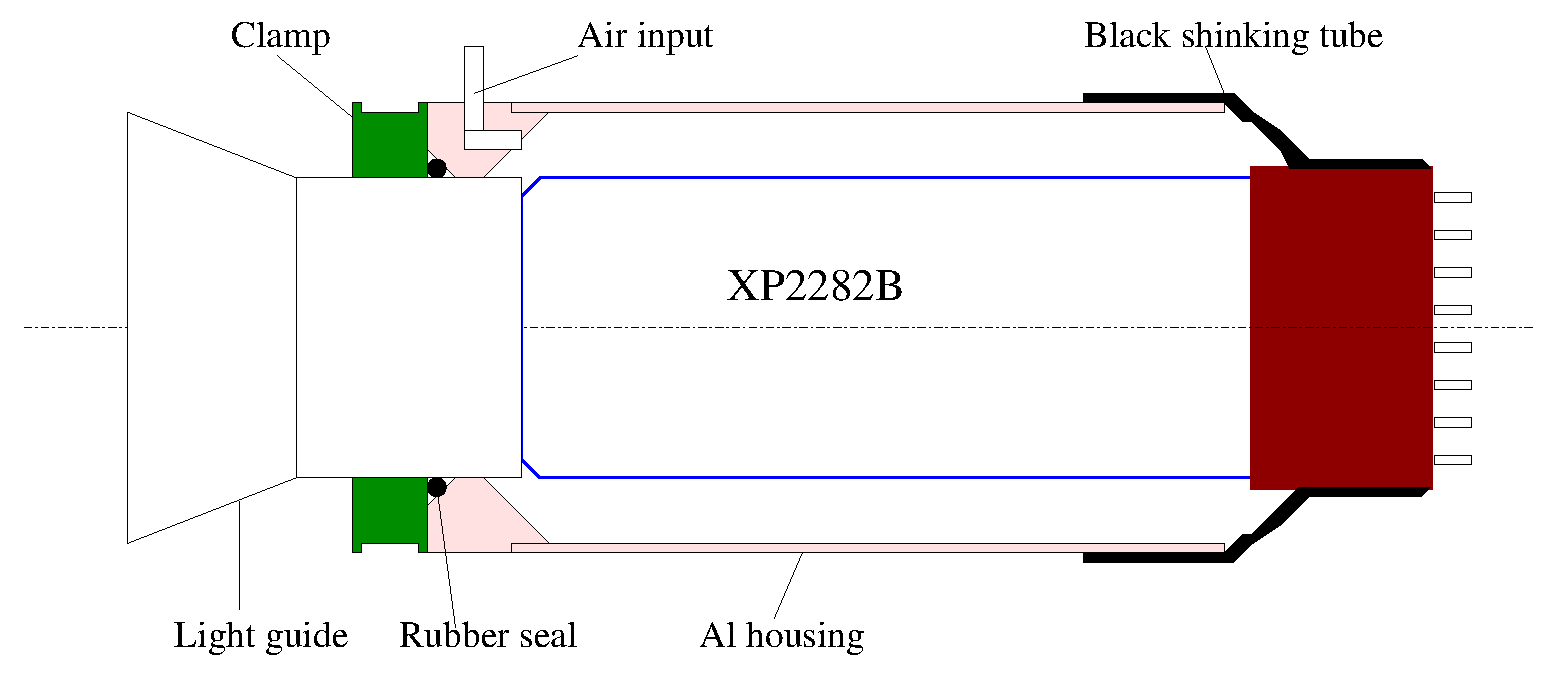
\includegraphics[width=.6\textwidth]{scint2_housing}
      \caption[Detectors: S2 PMT Housing]{Details of the PMT Housing for S2.}
      \label{fig:s2_pmt_housing}
    \end{center}
  \end{figure}
  
  There has been found in the past large He concentrations in Hall A, which
  can lead to a dramatic reduction in the PMT lifetime. To mitigate this
  problem, each PMT for S0, S1 and S2 is enclosed in a hermetic housing. Air from
  outdoors is supplied to the housing at a slight
  over-pressure. Figure~\ref{fig:s2_pmt_housing} shows a schematic of the
  housings used for the S2 PMTs.
}

\infolevthree{
  \section{ 2" PMT Bases for S1 Trigger Counters}
  
  A schematic diagram of the 2" PMT Base is shown in
  Figure~\ref{fig:scint_1}.  The Base consists of three main components.
  These are the front tubular housing (06), which encloses the PMT, part of
  the scintillator counter's light guide (01), and the mu-metal shield
  (10). The actual base with the socket and the dynode chain is a separate
  part, actually an assembly of parts (09-19). The rear tubular housing (07)
  completes the assembly and encloses the dynode chain and wiring. The three
  main sections join at the coupling nut (14), which threads partly inside
  the front tubular housing, while the rear tubular housing threads on the
  remaining part.
  
  The PMT and the electronic amplification components are mounted on a
  P.C. board (15) which is enclosed in an aluminum Faraday cage. This assures
  rigidity and protection from stray RF fields. The mu-metal shield is at
  cathode potential to minimize the dark current due to capacitive discharge
  in the photo cathode glass window.
  
  \begin{figure}[tbhp]
    \begin{center}
      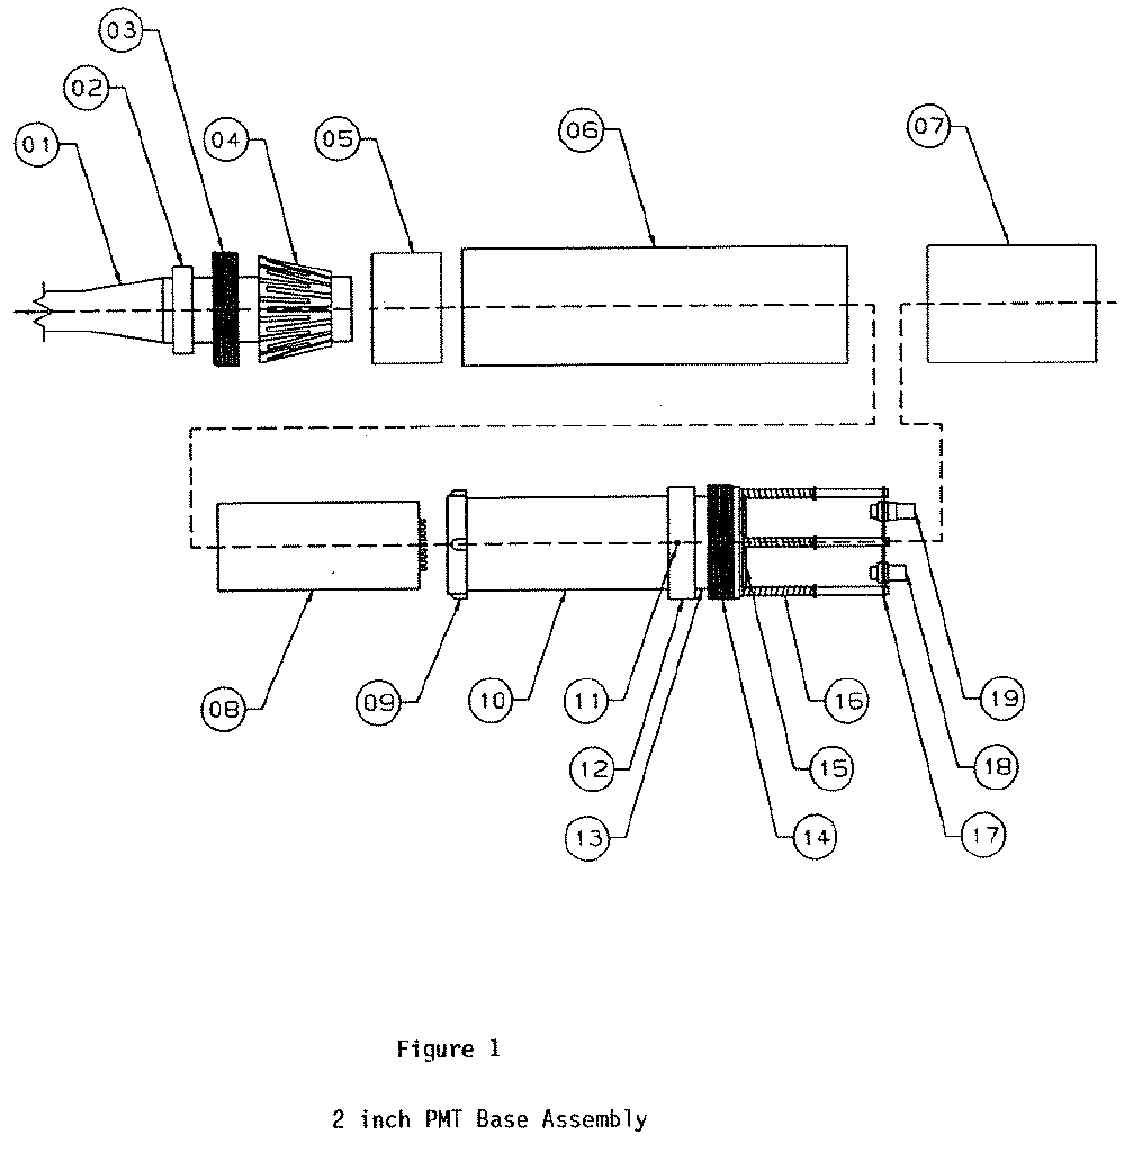
\includegraphics[angle=0,width=.6\textwidth]{scint_fig1}
      \caption[Detectors: 2'' PMT Base]{The 2" PMT base used in S1 trigger
	scintillators.}
      \label{fig:scint_1}
    \end{center}
  \end{figure}

  \paragraph{The Electronic Amplification Chain}
  \begin{figure}[tbhp]
    \begin{center}
      
\includegraphics[angle=0,width=.8\textwidth]{scint_fig2a}
      \caption[Detectors: 2'' PMT Base]{The 2" PMT base used
	in the S1 trigger scintillators.}
      \label{fig:scint_2}
    \end{center}
  \end{figure}
  
  
  The arrangement of the resistor dynode chain is shown in 
  Figure~\ref{fig:scint_2}. The 
  cathode is connected to the mu-metal shield through a 10 M$\Omega$ resistor, in
  addition to the 1 M$\Omega$ resistor between the cathode and the negative HV. The
  dynode chain incorporates an adjustable potentiometer (0-500 $\Omega$) to allow a
  match between the PMT and the external load, in order to eliminate after-pulse
  ringing.  This potentiometer should be adjusted at first to 250 $\Omega$ and then
  make fine adjustments as needed by observing the anode pulses on the
  oscilloscope for critical matching. It is not advisable to do the adjustments
  with HV on. Instead, the process should be done with HV off; remove the rear
  tubular housing, adjust the potentiometer, replace the rear housing, and then
  turn the HV on again. Iterate until the matching is accomplished. In addition to the
  obvious safety concerns, one does not want to remove the light sealing rear
  housing from an active PMT and induce a large light leak which could destroy
  the PMT. 
  
  The bases have been extensively tested under beam conditions. 
  They have several safety related features but these cannot protect anyone who 
  is bent on violating operating procedures and common sense. They allow the 
  removal of the PMT/Base assembly, for repairs of the electronics or replacement 
  of a PMT, without decoupling the housing and collets from the light guide. 
  Thus, replacement of PMTs can be done in minutes without the need to remove the 
  scintillator counters from their subframes.
}

\section{Safety Assessment}
  
\begin{safetyen}{10}{10}
  WARNING: The bases are high voltage devices: the high voltage should be
  turned off before handling.
  
  The maximum (negative) voltage for both the PMTs and dynode chain is 3 kV. In actual 
  use, however, there should be no need to exceed the 1.8-2.1 kV operating 
  parameters, since both PMTs and dynode chain have high gain. Nevertheless, the 
  bases are high voltage devices and care should be exercised during handling and 
  setup. The external aluminum parts, the front and rear housing, and the back 
  plate (17), are all grounded via the ground of the BNC (18) and SHV (19) 
  connectors. Since the back plate is connected to the coupling nut via the three 
  steel posts, the front plate is also grounded via the coupling nut and the back 
  plate. Common sense, however, dictates that the bases are not to be handled     
  while under high voltage, even when multiple grounding connections are provided.
  
  The mu-metal shield is also under high voltage, since it is connected to the 
  cathode. Electrical isolation between the mu-metal shield and the front 
  tubular housing is assured by the high dielectric retainer ring (12) and the 
  plastic insulator (09) at the free end of the mu-metal shield. The air gap 
  between the mu-metal shield and the front tubular housing is 6 mm, thus the 
  breakdown value (18 kV) far exceeds the maximum 3.0 kV of the PMT.
  
  In the event that the mu-metal shield is inserted without the plastic insulator 
  ring, or some oaf decides to operate the base without the outside housings, the 
  11 M$\Omega$ resistors between the -HV and the mu-metal shield will restrict the 
  current flow through the mu-metal shield (and the oaf's hands) to less than 0.2 
  mA with 2.1 kV on the base. 
\end{safetyen}

\section{Responsible Personnel} 
The following individuals are responsible for operation of the trigger counters. 
\begin{itemize}
\item[~]Segal, Jack - x7242 
\item[~]Wojtsekhowski, Bogdan - x7191 
\end{itemize} 

% ===========  CVS info
% $Header: /group/halla/analysis/cvs/tex/osp/src/hrs_det/scin.tex,v 1.9 2003/12/13 06:23:38 gen Exp $
% $Id: scin.tex,v 1.9 2003/12/13 06:23:38 gen Exp $
% $Author: gen $
% $Date: 2003/12/13 06:23:38 $
% $Name:  $
% $Locker:  $
% $Log: scin.tex,v $
% Revision 1.9  2003/12/13 06:23:38  gen
% Septum added. Name tables. Polishing
%
% Revision 1.8  2003/12/05 07:12:10  gen
% shower.tex modified. infolevel added. Polishing
%
% Revision 1.7  2003/11/12 20:39:30  feuerbac
% typo fix
%
% Revision 1.6  2003/11/12 20:26:11  feuerbac
% A little more information about S0.
%
% Revision 1.5  2003/11/11 21:15:48  feuerbac
% Add line about S0, minor improvement to formatting.
%
% Revision 1.4  2003/11/11 20:13:58  feuerbac
% Updated scintillator text.
% Removed mention of S3 and the base-replacement procedure.
% Updated text and figures for S2's upgrade to S2m.
%
% Revision 1.3  2003/06/06 17:00:27  gen
% Revision printout changed
%
% Revision 1.2  2003/06/05 23:30:01  gen
% Revision ID is printed in TeX
%
% Revision 1.1.1.1  2003/06/05 17:28:30  gen
% Imported from /home/gen/tex/OSP
%
%  Revision parameters to appear on the output
